% DOCUMENT TYPE: PRESENTATION
\documentclass[12pt,aspectratio=169]{beamer}

% PACKAGES TO USE
\usepackage[utf8]{inputenc}
\usepackage[spanish]{babel}
\usepackage{lastpage}
\usepackage{subcaption}
\usepackage[export]{adjustbox}

% CONFIGURATIONS
\setbeamertemplate{footline}[frame number]
\captionsetup{justification=centering}

% PRESENTATION INFO
\title[Red Neuronal Convolucional Adversarial]{Reconstrucción de Huellas Dactilares Digitales Utilizando un Modelo Generativo Adversarial Convolucional}
\author[Andrade, C]{Cristian Yesid Andrade Hernández}
\institute[Universidad de los Andes]
{ 
\includegraphics[width=5cm]{figs/uniandes_logo.png} }

\date{\today}

% DOCUMENT
\begin{document}

% ==== INIT SLIDE ====
\frame[plain]{\titlepage}

% ==== SLIDE 2 ====
\begin{frame}{Introducción}

    La captura digital de huellas dactilares puede resultar en imágenes deterioradas.
    \vspace{3mm}

    \begin{figure}
        \begin{subfigure}{0.3\textwidth}
            \centering
            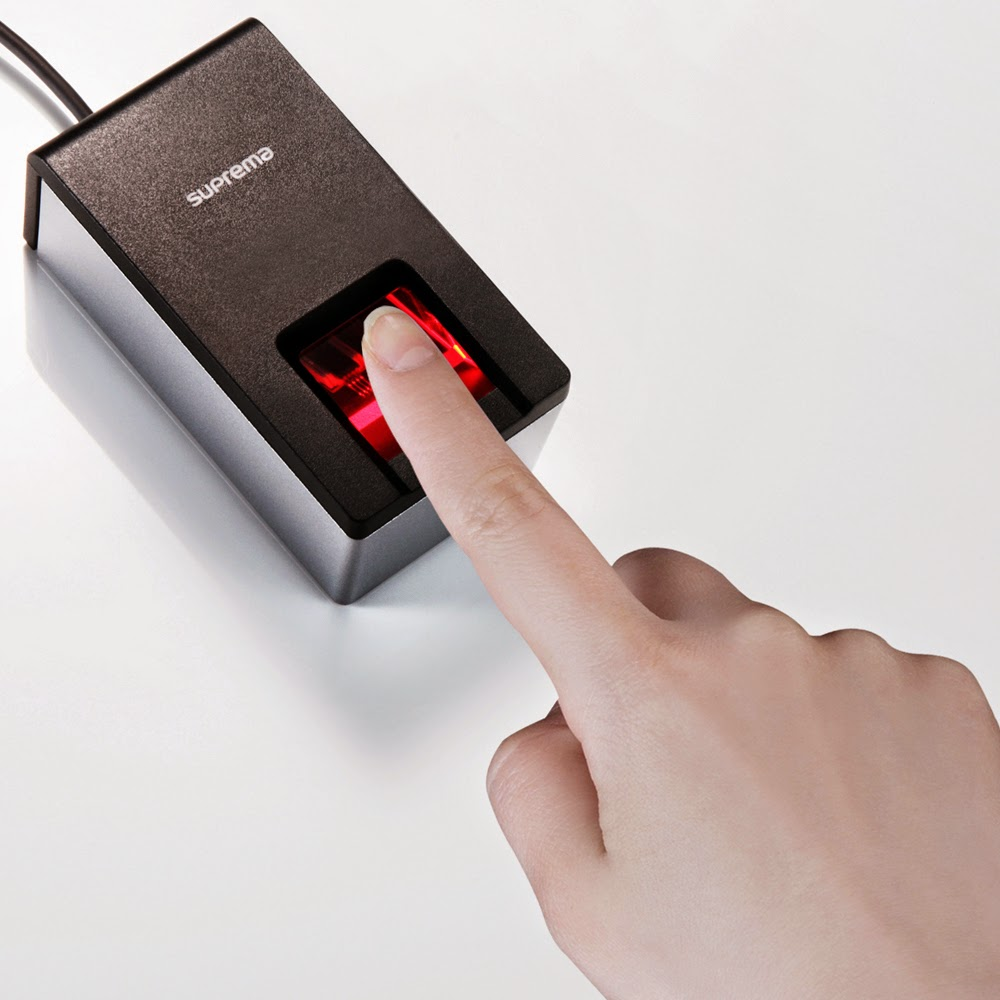
\includegraphics[scale=0.12]{figs/dedo_lector_biometrico.jpg}
        \end{subfigure}
        \begin{subfigure}{0.14\textwidth}
            \centering
            $\longrightarrow$
        \end{subfigure}
        \begin{subfigure}{0.23\textwidth}
            \centering
            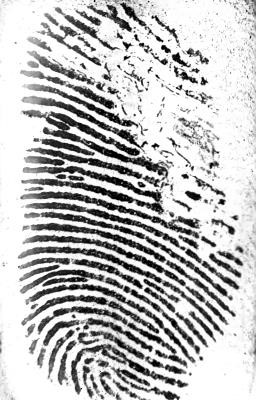
\includegraphics[scale=0.32]{figs/deteriorada_1.jpg}
            \caption{Huella incompleta}
        \end{subfigure}
        \begin{subfigure}{0.23\textwidth}
            \centering
            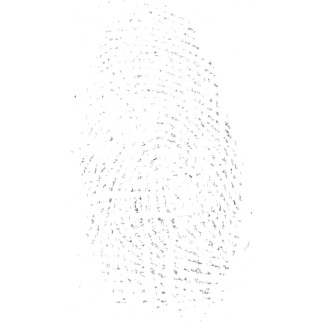
\includegraphics[scale=0.3]{figs/deteriorada_0.png}
            \caption{Huella borrosa}
        \end{subfigure}
    \end{figure}

\end{frame}

% ==== SLIDE 3 ====
\begin{frame}{Red neuronal convolucional}

    Se propone reconstruir y mejorar la huella digital obtenida mediante una red neuronal convolucional.
    \vspace{5mm}

    \begin{figure}
            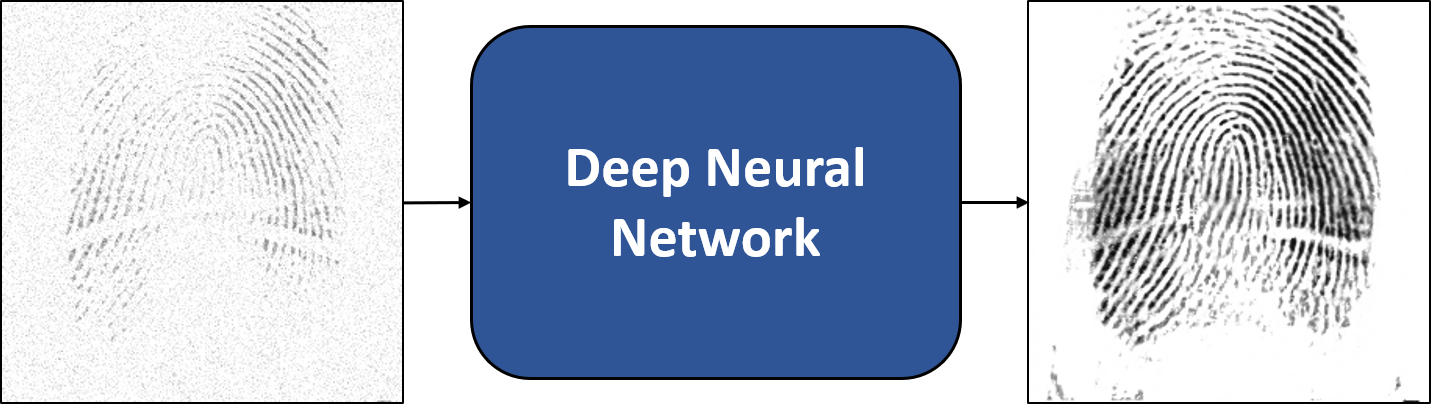
\includegraphics[scale=0.38]{figs/end_to_end.png}
            \caption{Modelo end to end}
    \end{figure}

\end{frame}

% ==== SLIDE 4 ====
\begin{frame}{Modelos Generativos Adversariales}

    \begin{figure}
        \begin{subfigure}{0.48\textwidth}
            \centering
            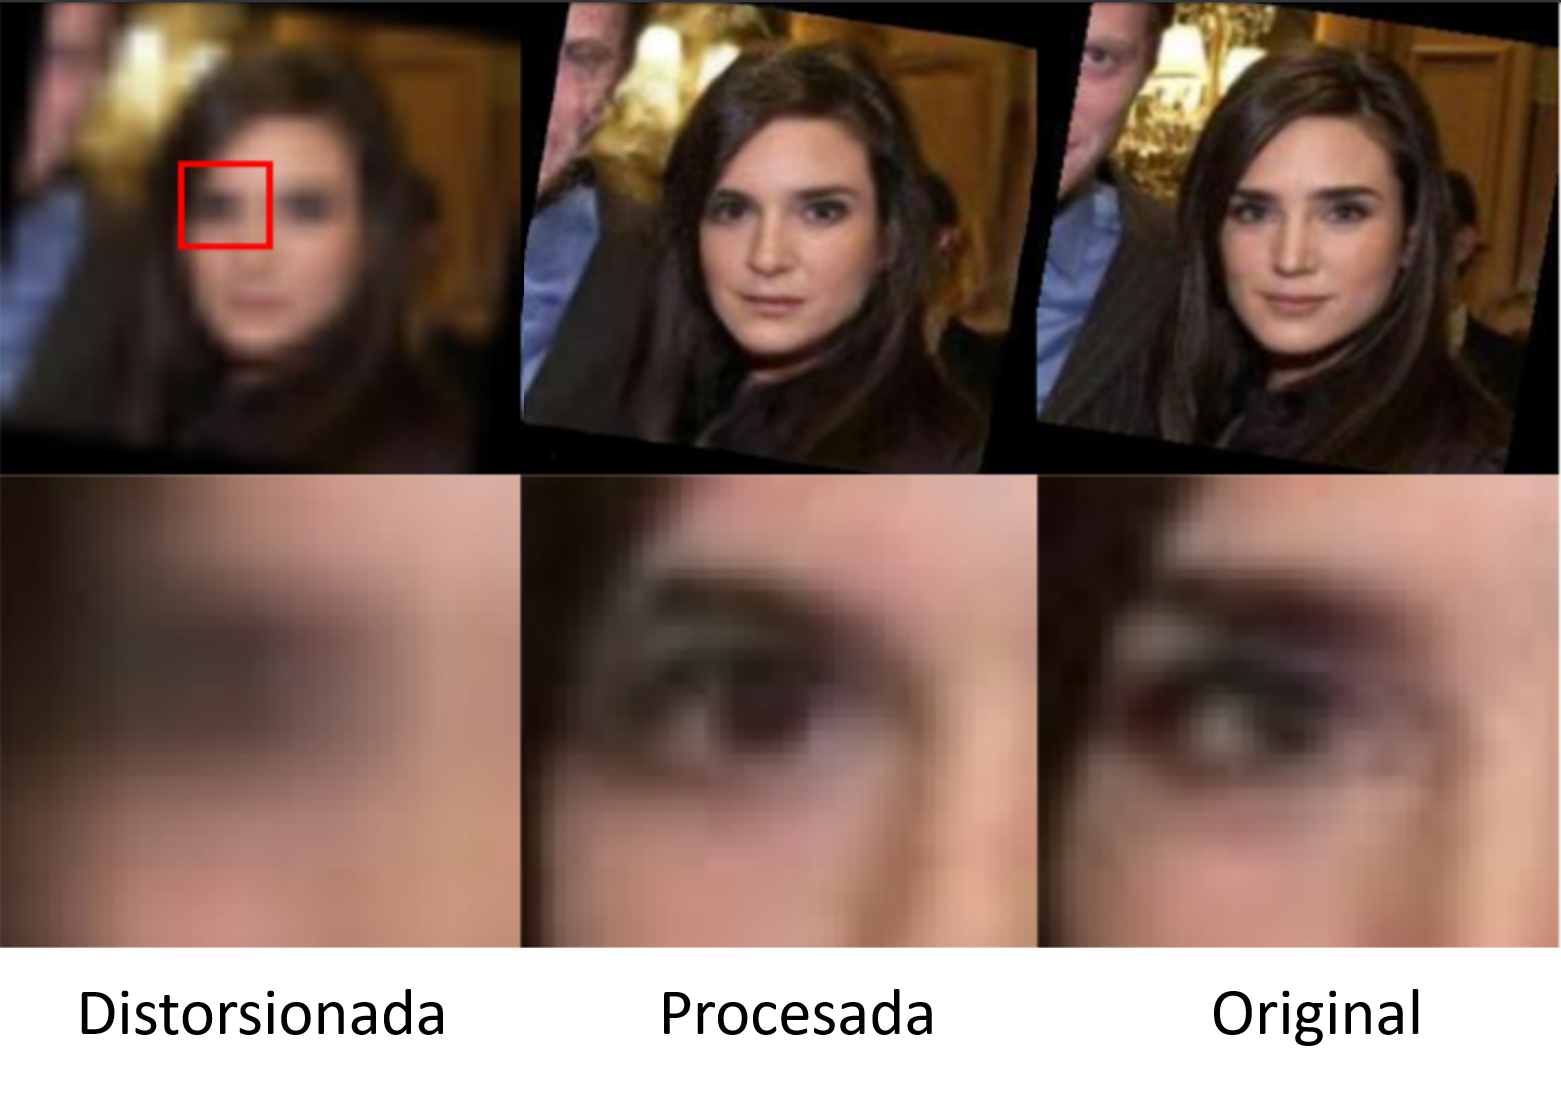
\includegraphics[scale=0.23]{figs/superresolution_example.png}
            \caption{Súper resolución}
        \end{subfigure}
        \begin{subfigure}{0.48\textwidth}
            \centering
            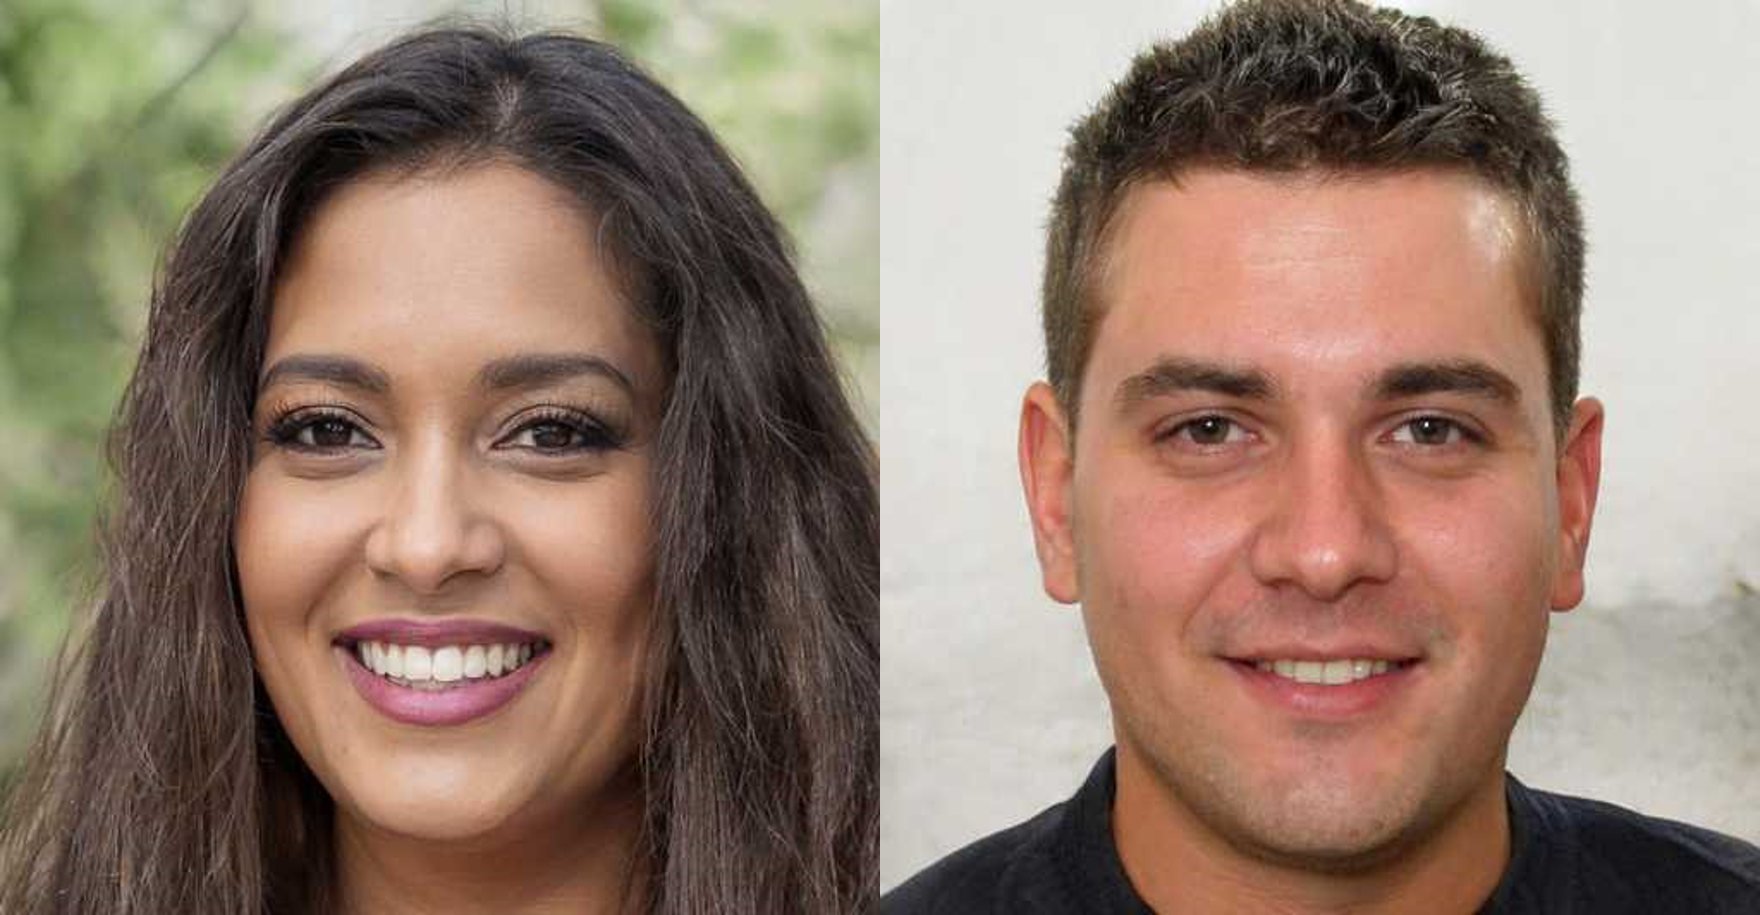
\includegraphics[scale=0.23]{figs/personas_inexistentes.png}
            \caption{Personas inexistentes}
        \end{subfigure}
    \end{figure}

\end{frame}

% ==== SLIDE 4 ====
\begin{frame}{Imagen digital}

    Composición de imagen digital de un canal.

    \begin{figure}
        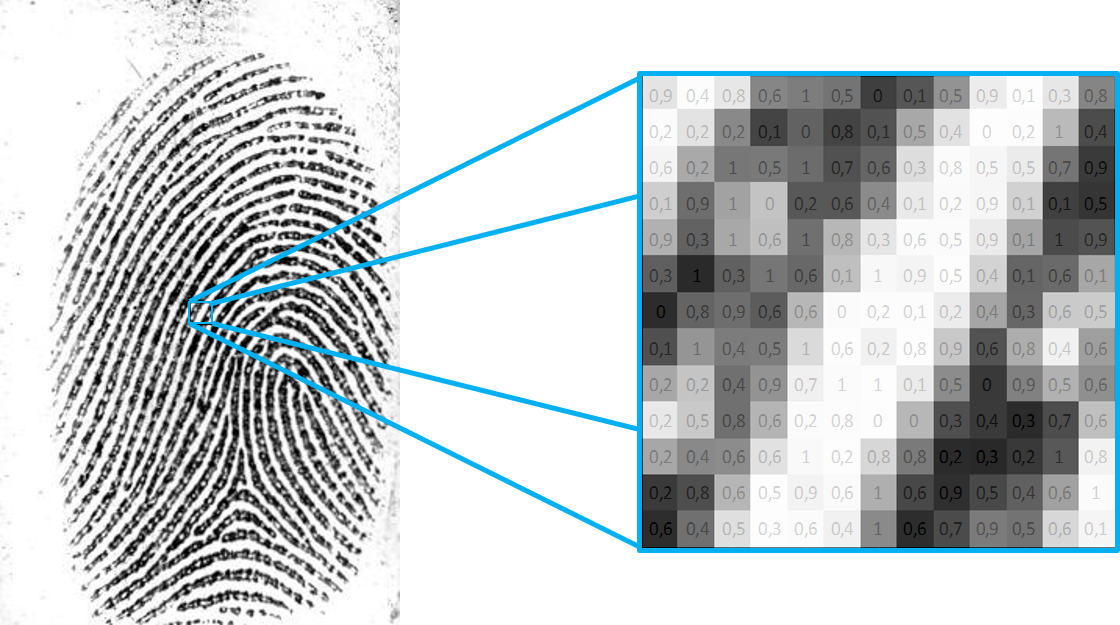
\includegraphics[scale=0.45]{figs/huella_pixeles_numeros.png}
        \caption{Huella dactilar digital}
    \end{figure}

\end{frame}

% ==== SLIDE 5 ====
\begin{frame}{Convolución}

    \begin{columns}[c] 
        \column{.42\textwidth}
            \begin{figure}
                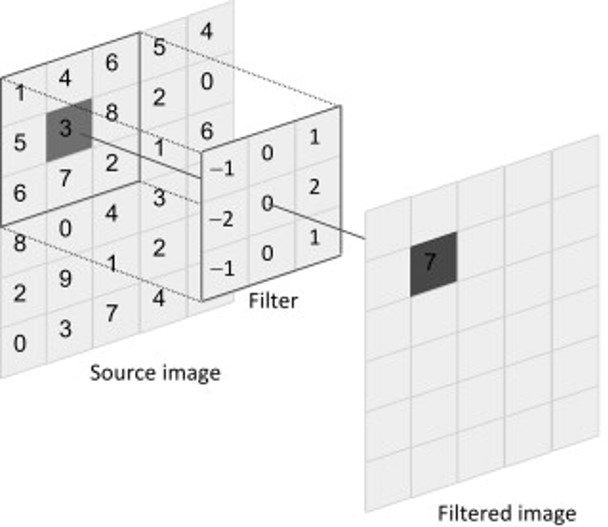
\includegraphics[scale=0.4]{figs/conv_2d.jpg}
                \caption{Proceso de convolución}
            \end{figure}
        \column{.58\textwidth}
            \begin{itemize}
                \item Características de bajo y alto nivel.
                \vspace{4mm}
                
                \begin{figure}
                    \begin{subfigure}{0.21\textwidth}
                        \centering
                        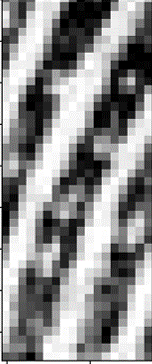
\includegraphics[scale=0.1]{figs/fll_0.png}
                        \caption{Cresta vertical}
                    \end{subfigure}
                    \begin{subfigure}{0.21\textwidth}
                        \centering
                        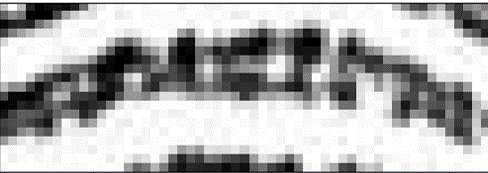
\includegraphics[scale=0.1]{figs/fll_1.png}
                        \caption{Cresta horizontal}
                    \end{subfigure}
                    \begin{subfigure}{0.21\textwidth}
                        \centering
                        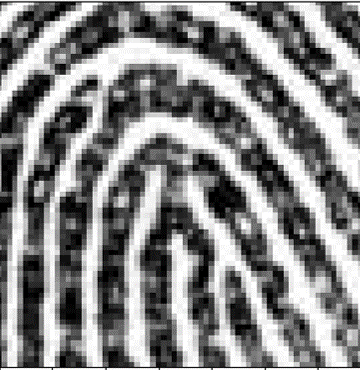
\includegraphics[scale=0.1]{figs/fhl_0.png}
                        \caption{Núcleo}
                    \end{subfigure}
                    \begin{subfigure}{0.21\textwidth}
                        \centering
                        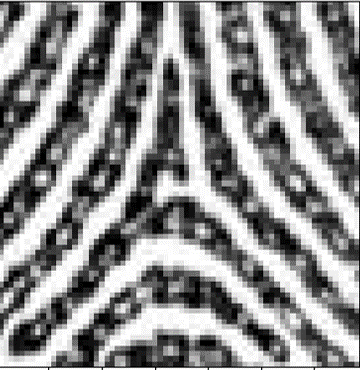
\includegraphics[scale=0.1]{figs/fhl_1.png}
                        \caption{Delta}
                    \end{subfigure}
                \end{figure}
                \vspace{3mm}
                
            \end{itemize}
    \end{columns}

\end{frame}

% ==== SLIDE 6.1 ====
\begin{frame}{Modelo de reconstrucción}

   \begin{figure}
        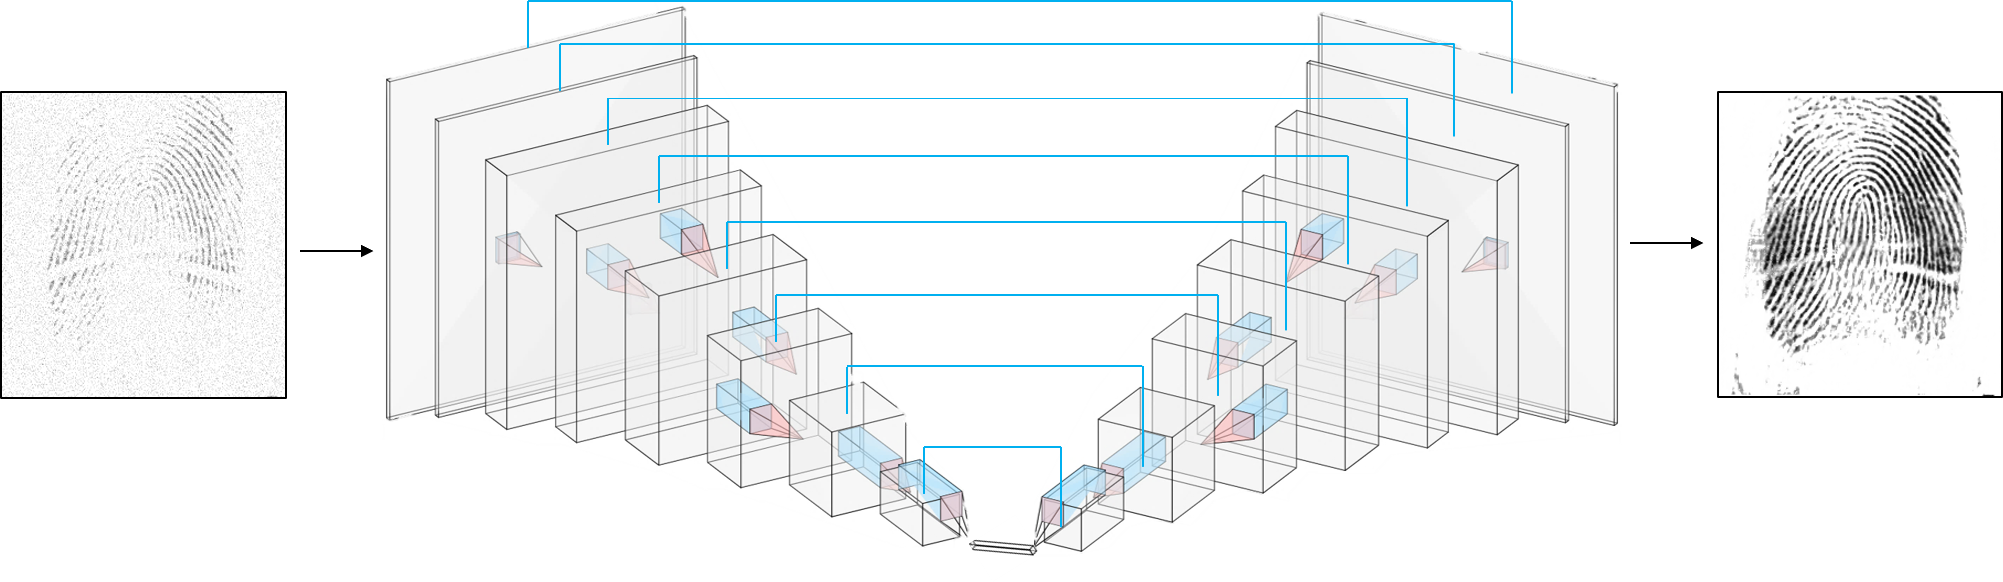
\includegraphics[scale=0.4]{figs/layers_nn_two.png}
        \caption{Componente convolucional de restauración}
    \end{figure}

\end{frame}

% ==== SLIDE 6.2 ====
\begin{frame}{Arquitectura Adversarial}

   \begin{figure}
        \begin{subfigure}{0.54\textwidth}
            \centering
            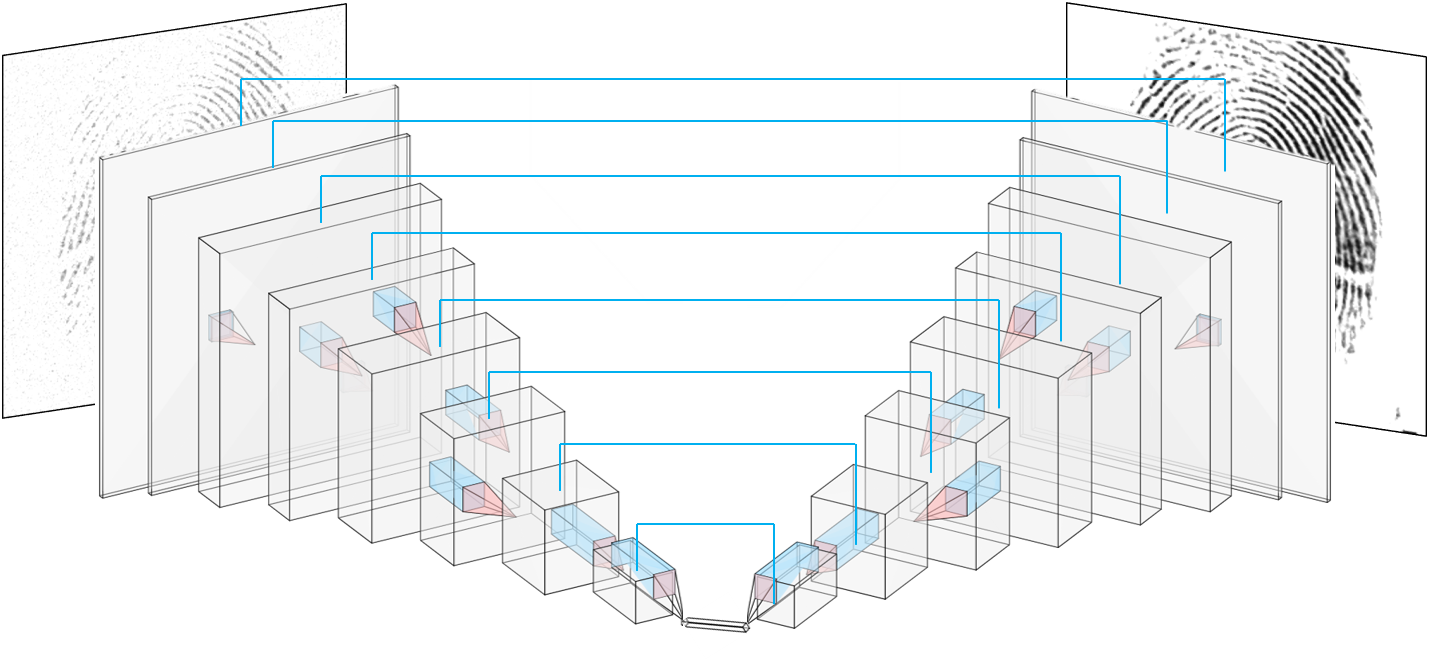
\includegraphics[scale=0.3]{figs/layers_nn_u.PNG}
            \caption{Componente que reconstruye y mejora las huellas \\ (Generador)}
        \end{subfigure}
        \begin{subfigure}{0.1\textwidth}
            \centering VS
        \end{subfigure}
        \begin{subfigure}{0.3\textwidth}
            \centering
            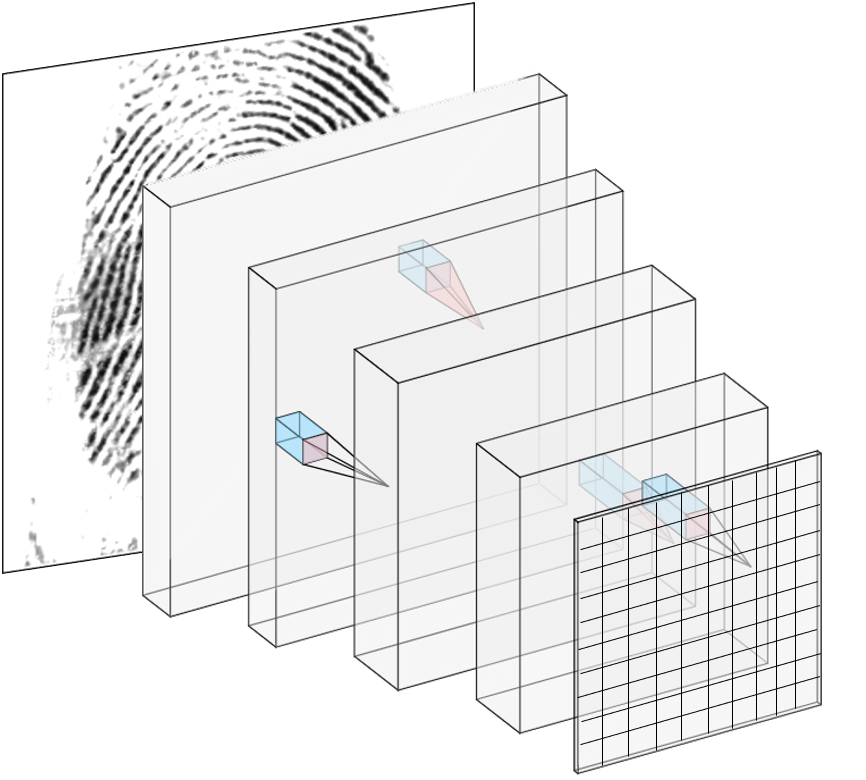
\includegraphics[scale=0.22]{figs/disc_cuad.png}
            \caption{Componente de validación de huellas \\ (Discriminador)}
        \end{subfigure}
    \end{figure}

\end{frame}

% ==== SLIDE 7 ====
\begin{frame}{Funciones de costo}

    Costo del Generador:
    \begin{equation}
        - log(disc(x,gen(x)))+\alpha||y-gen(x)||_{[1]}
    \end{equation}
    Costo del Discriminador:
    \begin{equation}
        -log(1-disc(x,gen(x)))-log(disc(x,y))
    \end{equation}
    
    \vspace{5mm}
    
    El parámetro \textit{y} corresponde a la huella original, \textit{x} a la huella deteriorada y $\alpha$ define el peso del componente reconstructivo en la expresión.

\end{frame}

% ==== SLIDE 8 ====
\begin{frame}{Flujo de entrenamiento del modelo}

    \begin{figure}
        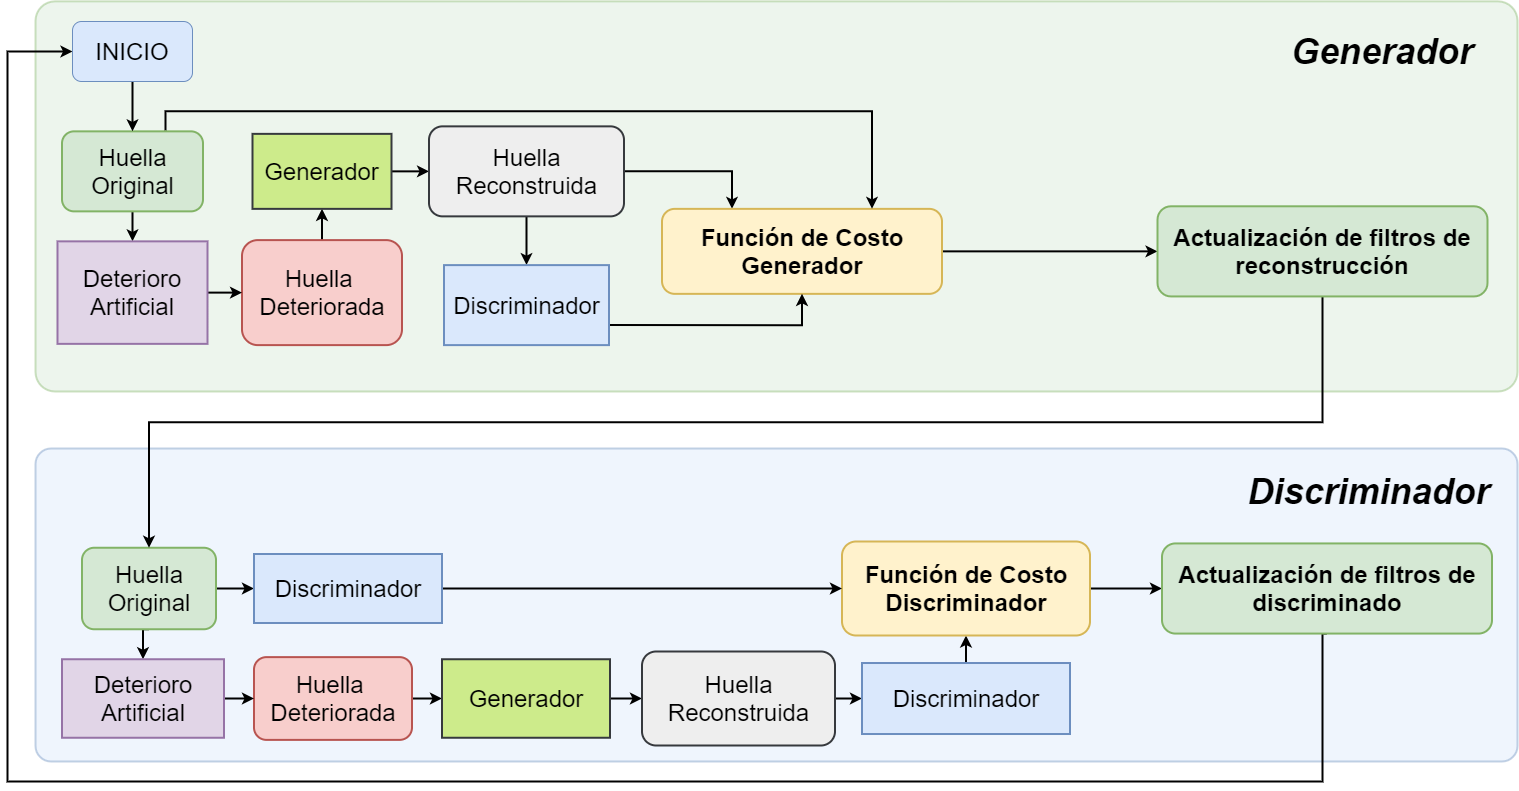
\includegraphics[scale=0.25]{figs/training_flow_overall.png}
    \end{figure}

\end{frame}

% ==== SLIDE 9 ====
\begin{frame}{Datos de entrenamiento, software y hardware}

    \begin{columns}[c] 
        \column{.7\textwidth}
            \begin{itemize}
                \item 100.000 Huellas proporcionadas por Olimpia.
                \vspace{3mm}
                \item Entrenamiento: 18.000 - Validación: 2.000
                \vspace{3mm}
                \item Software: Python y TensorFlow
                \vspace{3mm}
                \item Hardware: Cluster de cómputo de la Universidad de los Andes. Nvidia Tesla K40
                \vspace{3mm}
                \item Tiempo de entrenamiento: 1 día, 27 horas y 32 minutos.
            \end{itemize}
        \column{.3\textwidth}
            \begin{figure}
                
\includegraphics[scale=0.04]{figs/python}
            \end{figure}
            \vspace*{-4mm}
            \begin{figure}
                
\includegraphics[scale=0.3]{figs/tensorflow.png}
            \end{figure}
            \vspace*{-7mm}
            \begin{figure}
                
\includegraphics[scale=0.06]{figs/nvidia.png}
            \end{figure}
    \end{columns}

\end{frame}

% ==== SLIDE 10 ====
\begin{frame}{Deterioro Artificial}

    Las huellas dactilares fueron deterioradas artificialmente para conformar el dataset utilizado en el proceso de entrenamiento.
    \vspace{5mm}

    \begin{figure}
        \begin{subfigure}{0.48\textwidth}
            \centering
            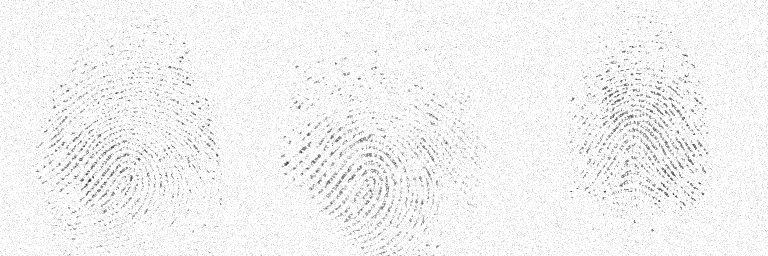
\includegraphics[scale=0.24]{figs/deterioration_2.png}
            \caption{Deterioro por factor externo}
        \end{subfigure}
        \begin{subfigure}{0.48\textwidth}
            \centering
            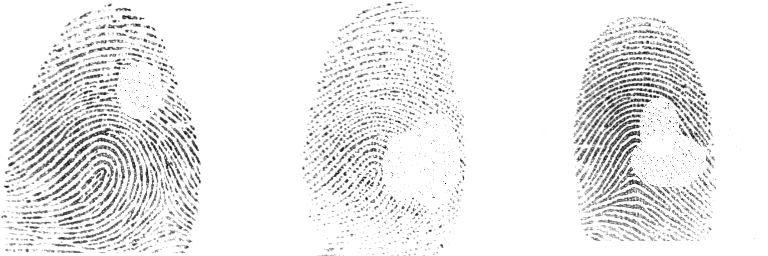
\includegraphics[scale=0.24]{figs/deterioration_1.png}
            \caption{Deterioro de la piel}
        \end{subfigure}
    \end{figure}

\end{frame}

% ==== SLIDE 11 ====
\begin{frame}{Curvas ROC y CMC}

    \begin{figure}
        \begin{subfigure}{0.48\textwidth}
            \centering
            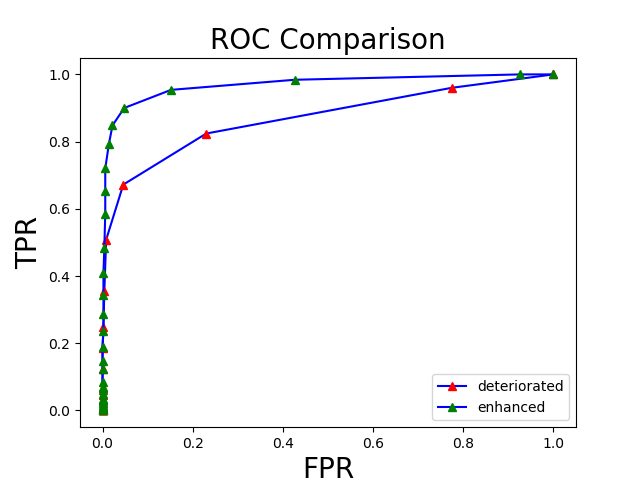
\includegraphics[scale=0.45]{figs/roc_comparison.png}
            \caption{Receiver operating characteristic}
        \end{subfigure}
        \begin{subfigure}{0.48\textwidth}
            \centering
            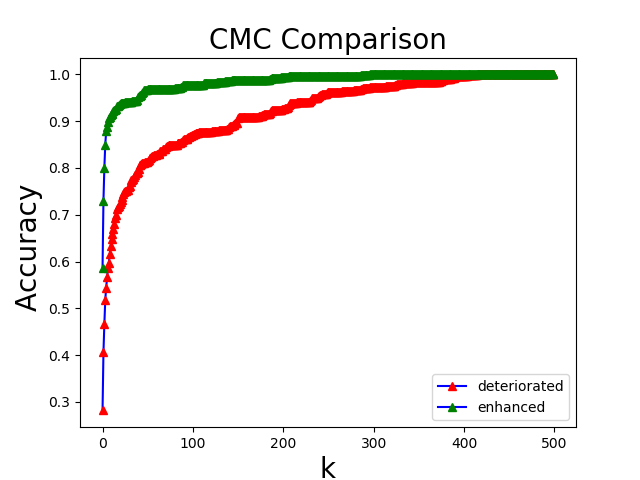
\includegraphics[scale=0.45]{figs/cmc_comparison.png}
            \caption{Cummulative match curve}
        \end{subfigure}
    \end{figure}

\end{frame}

% ==== SLIDE 12 ====
\begin{frame}{Calidad de las huellas}

    \begin{figure}
        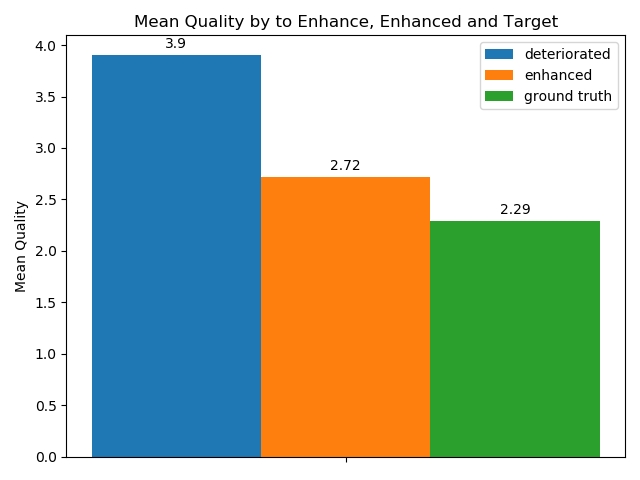
\includegraphics[scale=0.54]{figs/mean_qualities.png}
        \caption{Medida de calidad de las huellas}
    \end{figure}
    
\end{frame}

% ==== SLIDE 13 ====
\begin{frame}{Huellas restauradas}

    \begin{figure}
        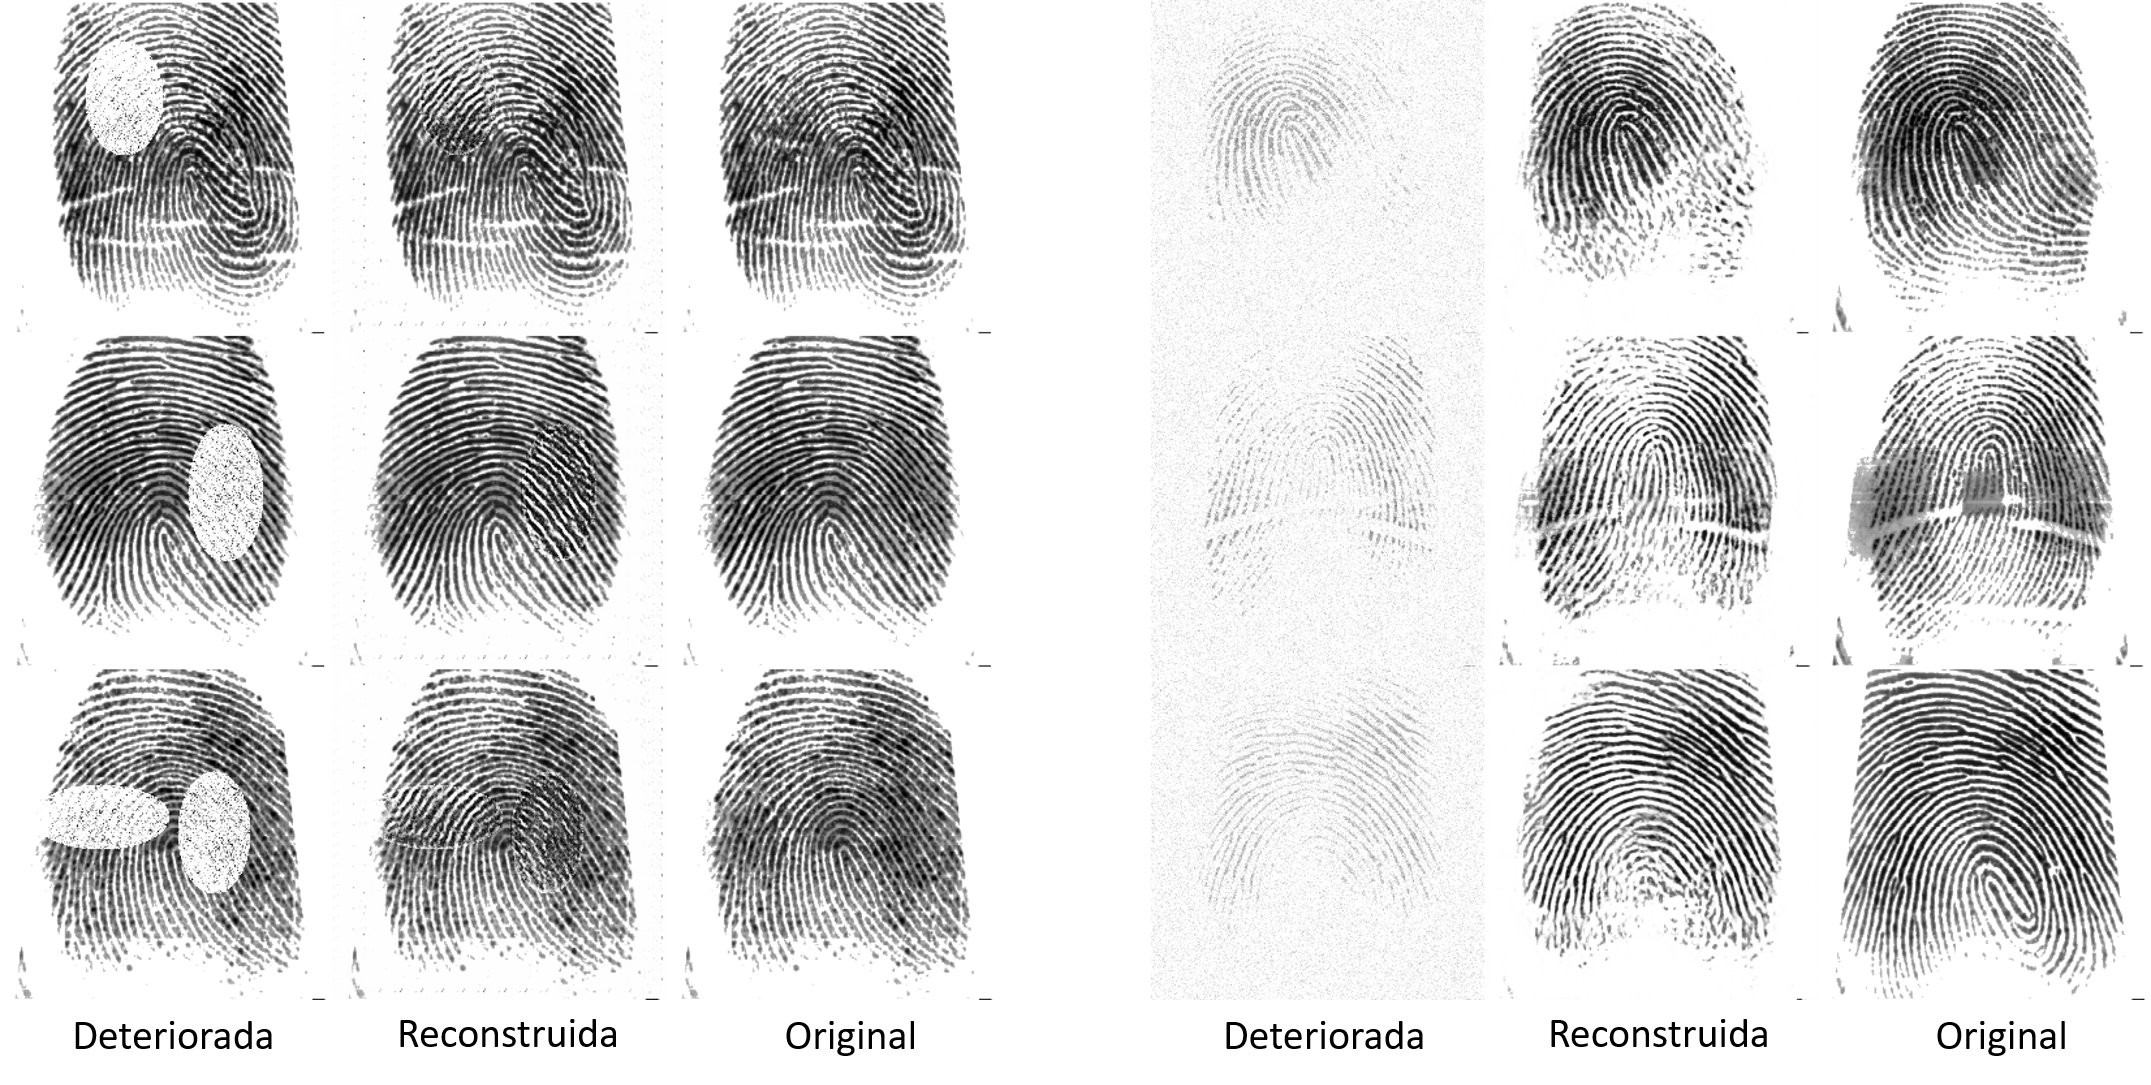
\includegraphics[scale=0.38]{figs/reconstruccion_labels.png}
    \end{figure}

\end{frame}

% ==== SLIDE 14 ====
\begin{frame}{Test de Carga Computacional}

    Restauración de 300 huellas dactilares.

    \begin{columns}[c] 
        \column{0.6\textwidth}
            \begin{figure}
            \begin{subfigure}{0.45\textwidth}
                \centering
                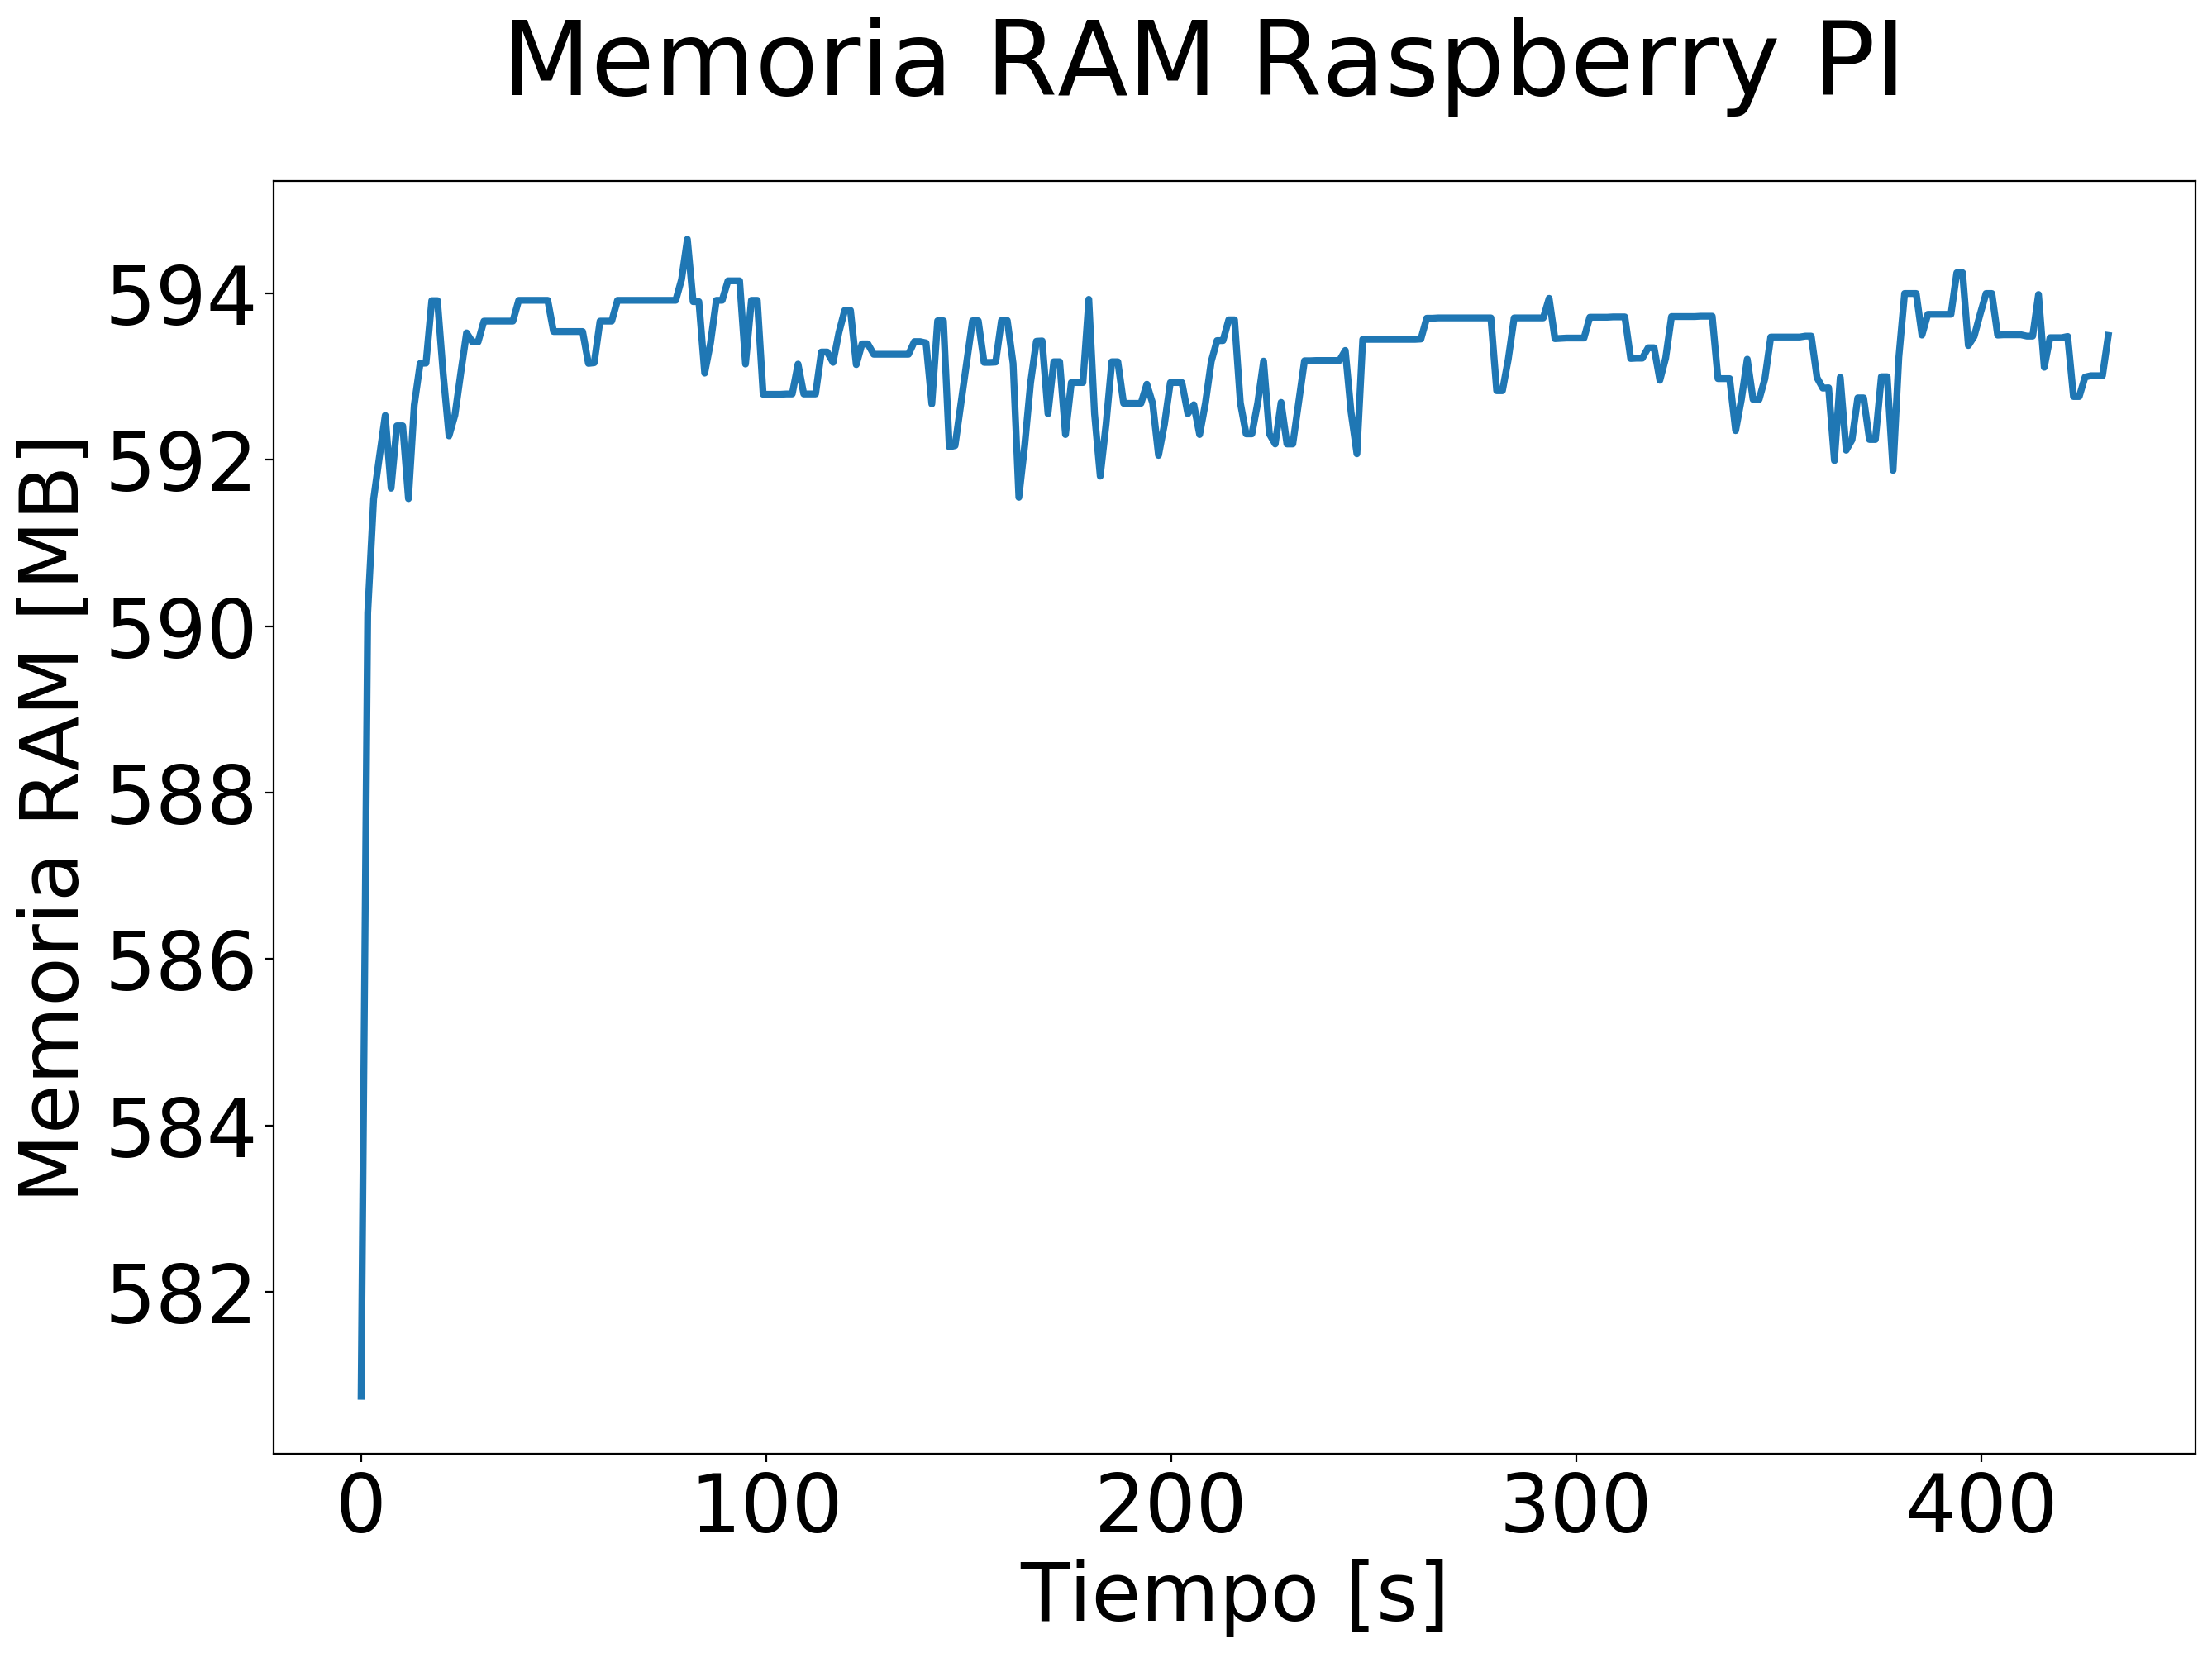
\includegraphics[scale=0.11]{figs/RAM RB.png}
                %\caption{RAM Raspberry PI}
            \end{subfigure}
            \begin{subfigure}{0.45\textwidth}
                \centering
                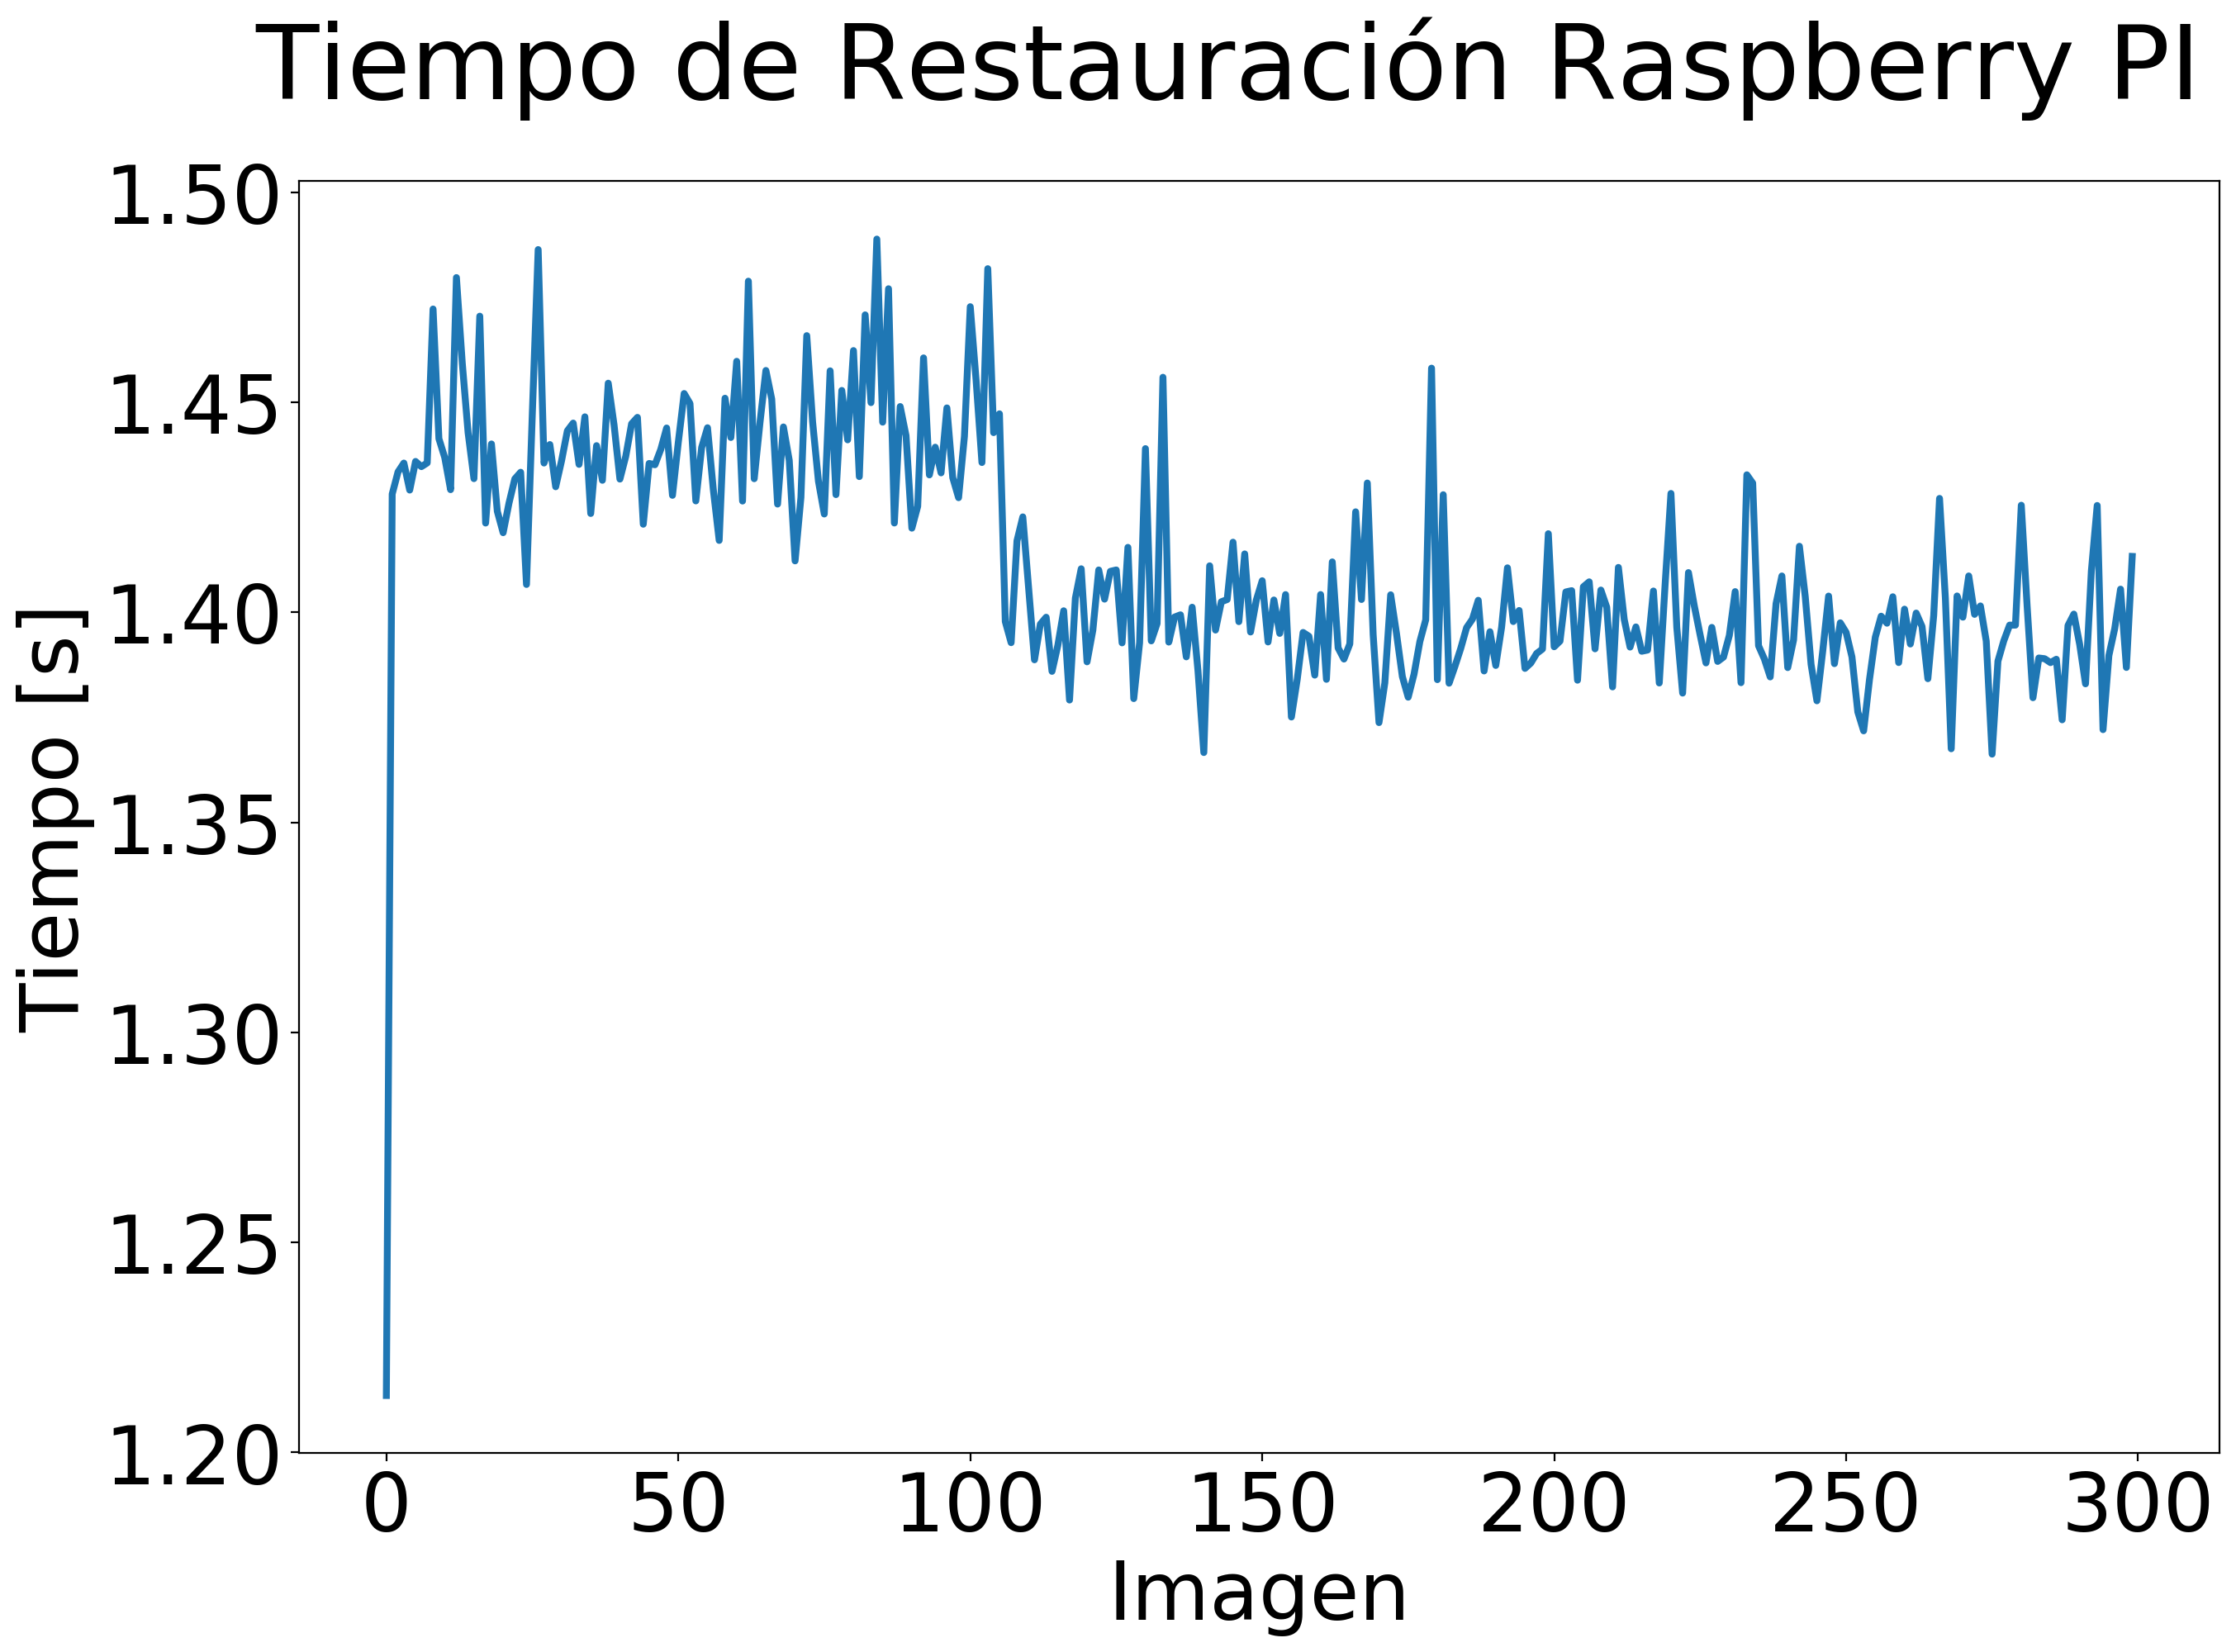
\includegraphics[scale=0.11]{figs/Tiempo RB.png}
                %\caption{Tiempo Raspberry PI}
            \end{subfigure}
            \\
            \begin{subfigure}{0.45\textwidth}
                \centering
                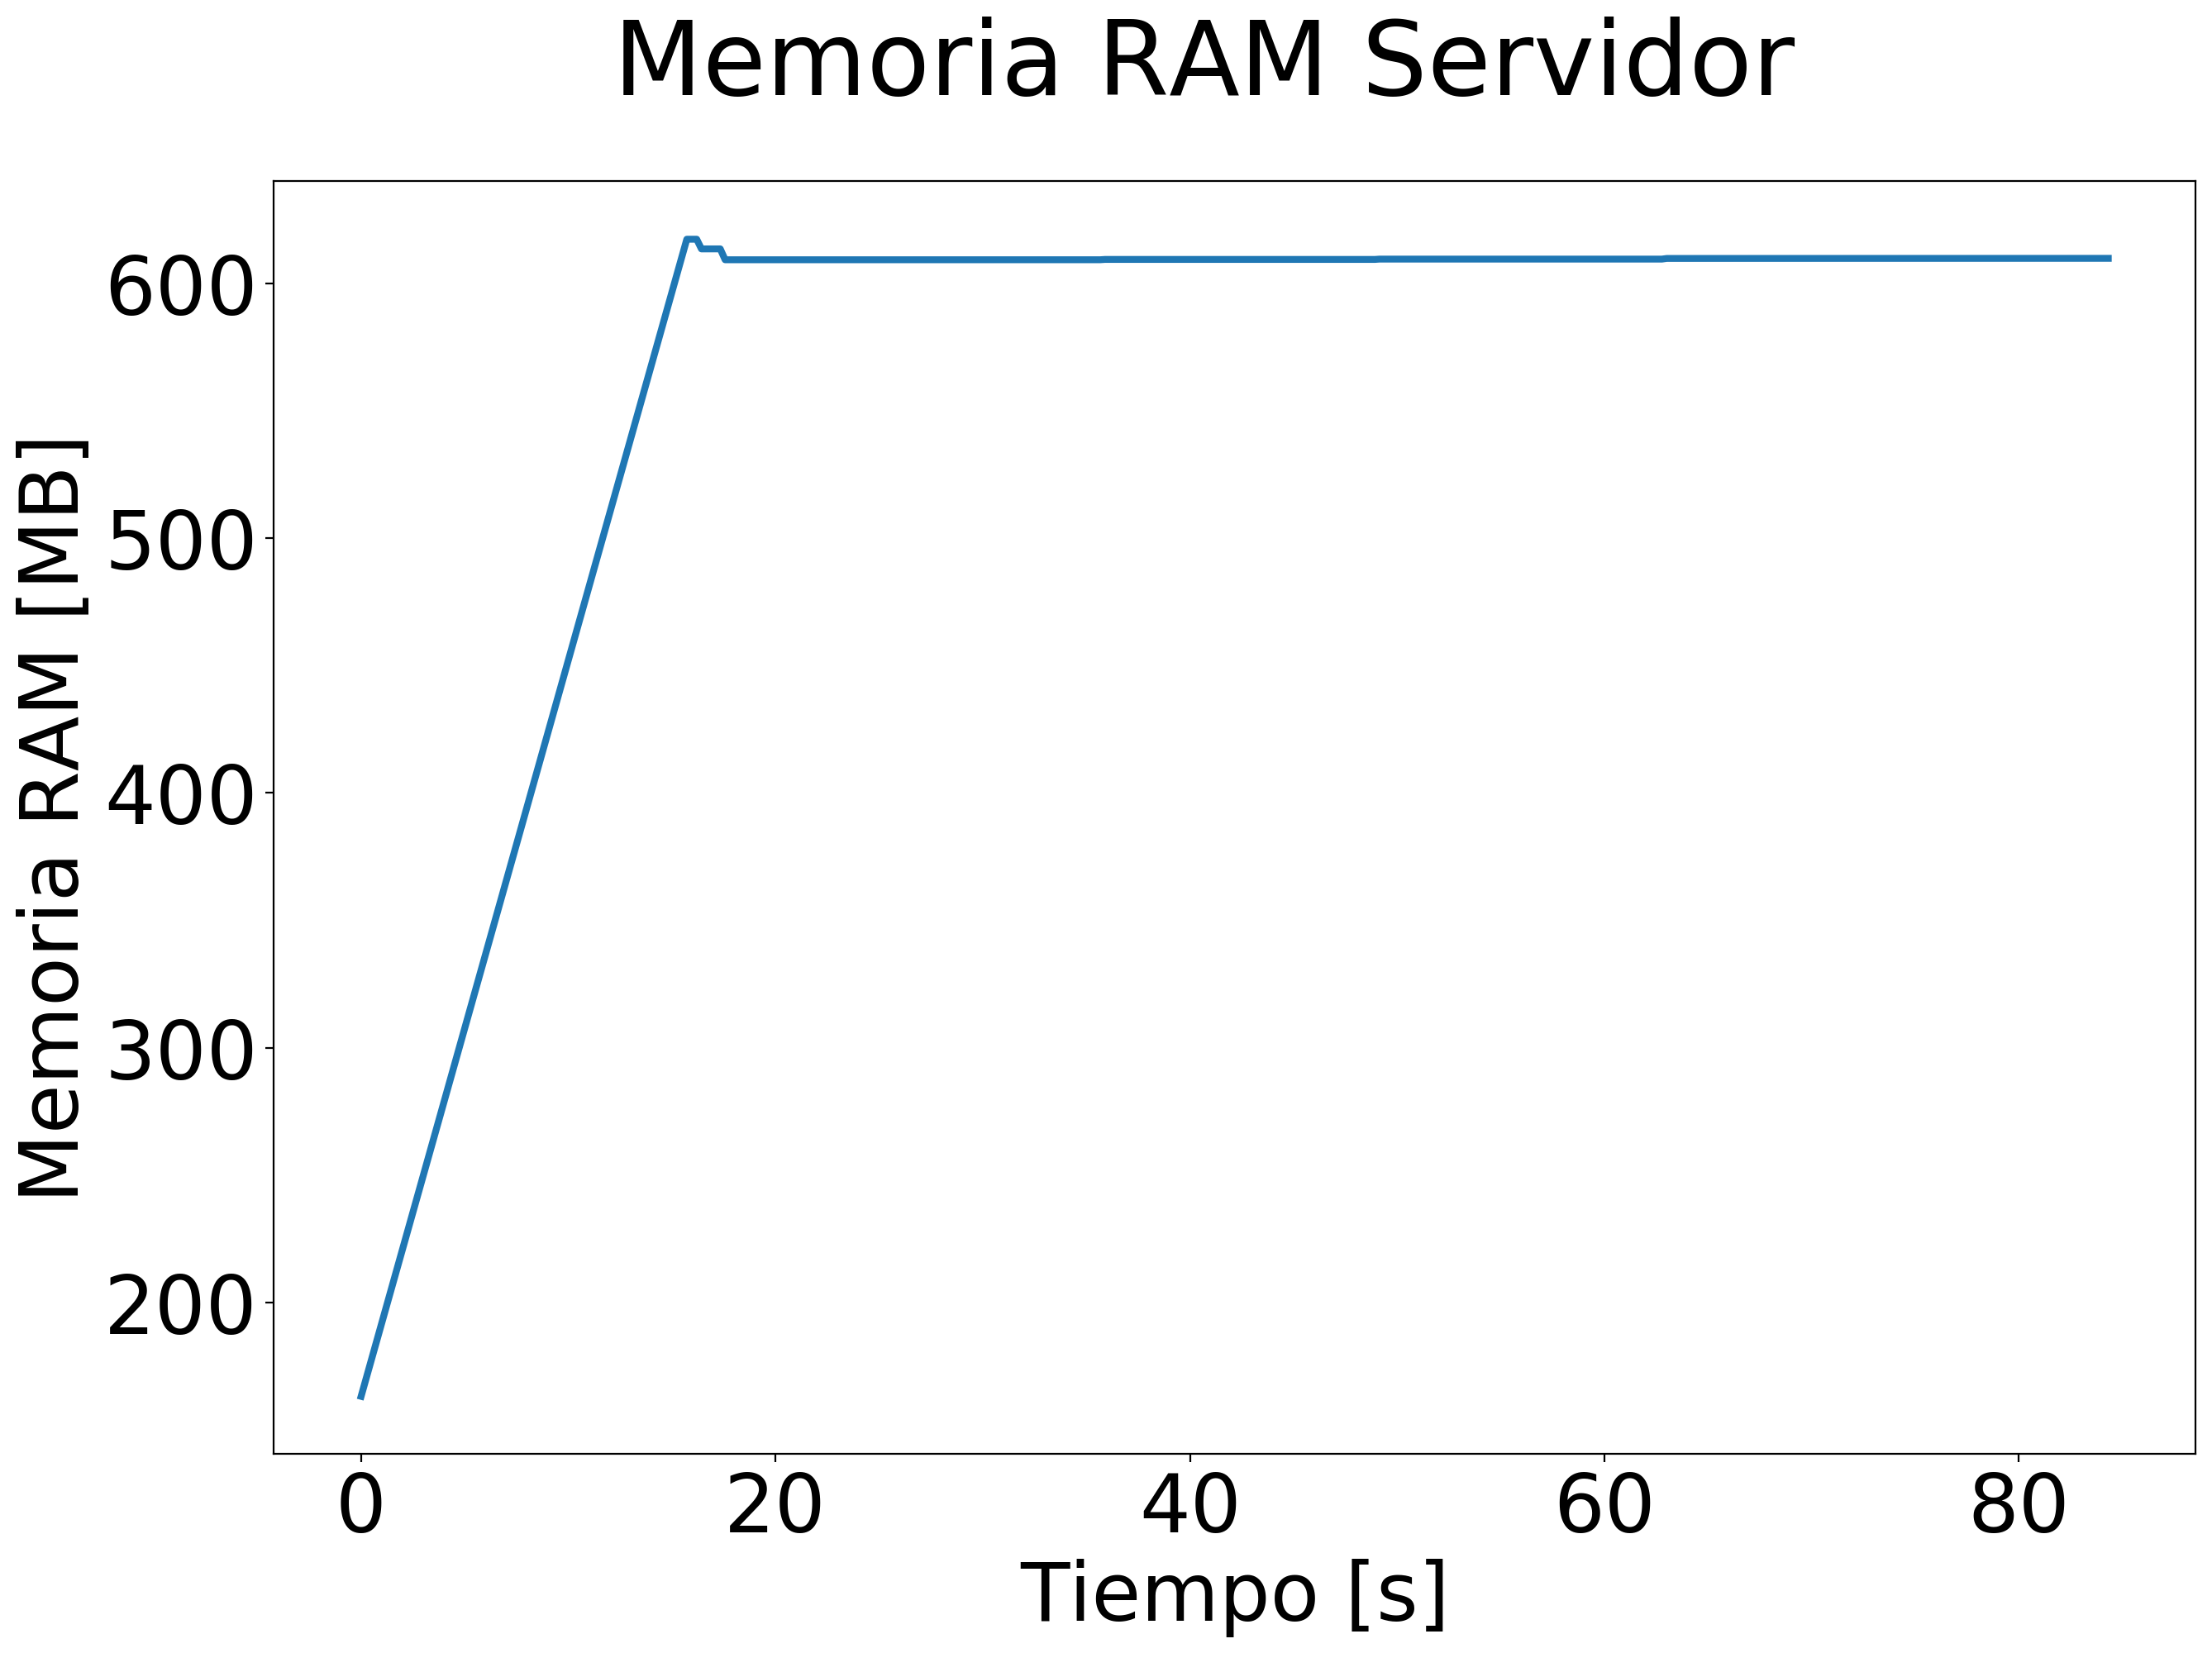
\includegraphics[scale=0.11]{figs/RAM Servidor.png}
                %\caption{RAM Servidor}
            \end{subfigure}
            \begin{subfigure}{0.45\textwidth}
                \centering
                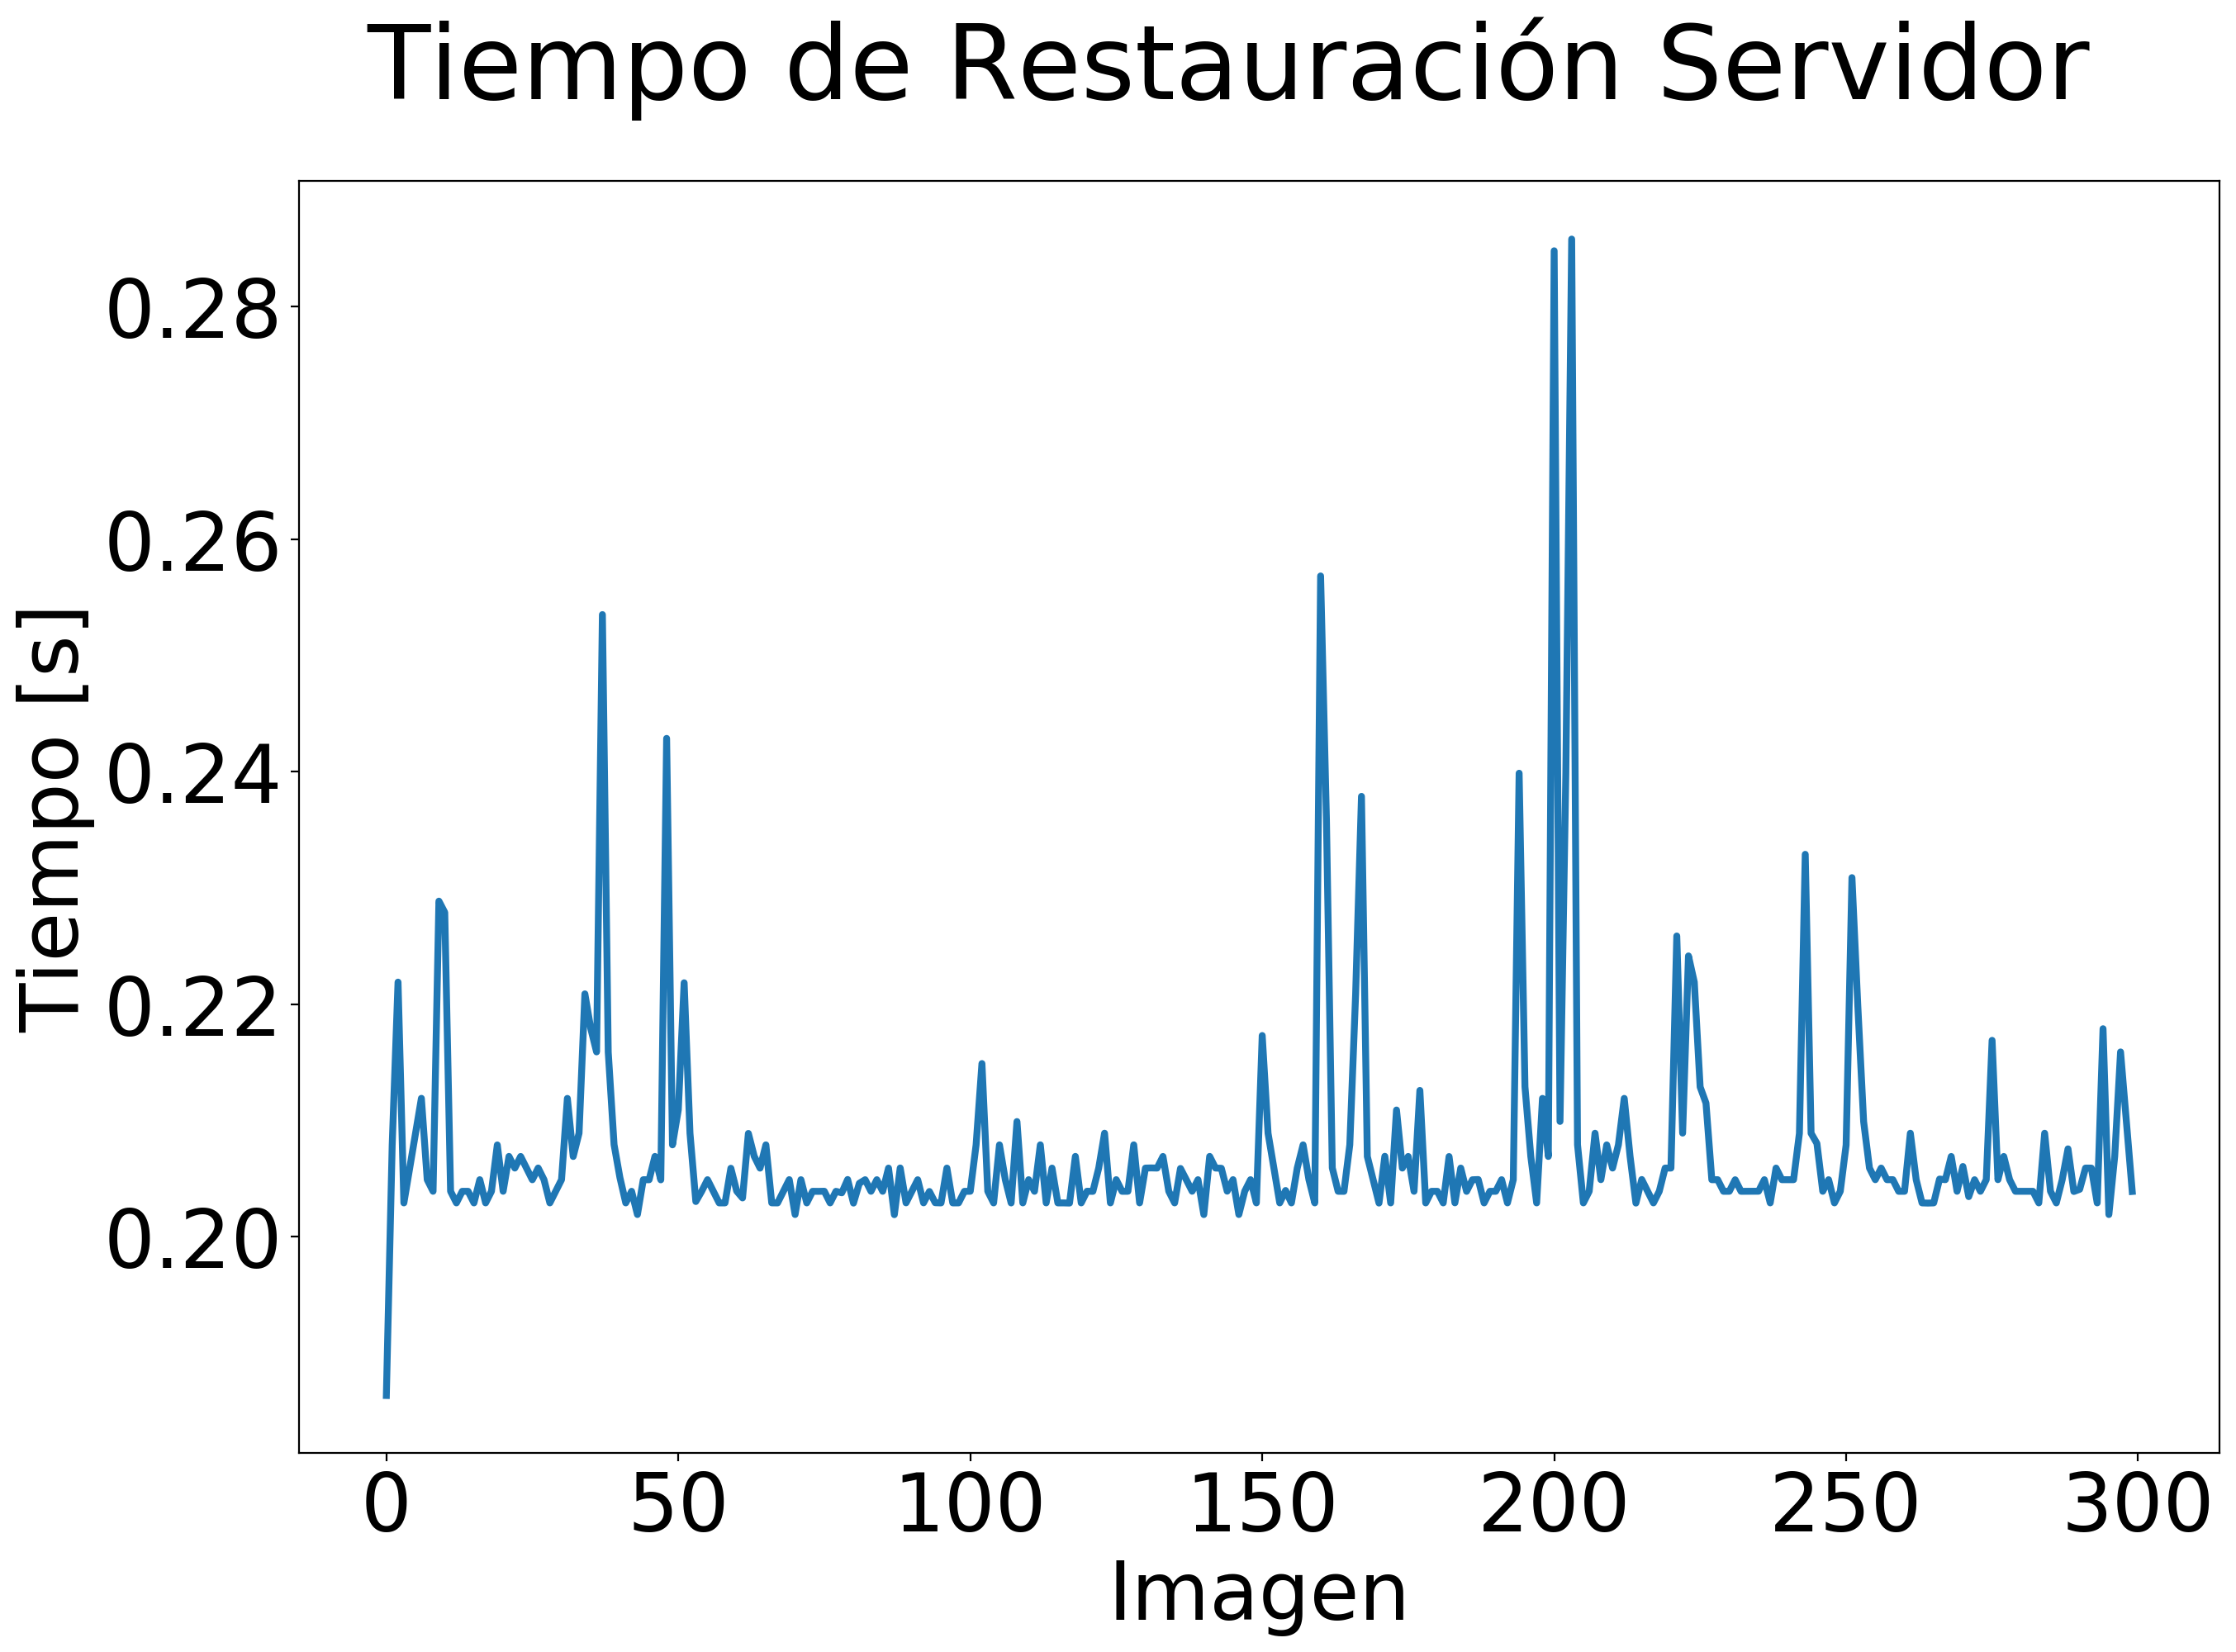
\includegraphics[scale=0.11]{figs/Tiempo Servidor.png}
                %\caption{Tiempo Servidor}
            \end{subfigure}
            \end{figure}
        \column{0.4\textwidth}
            Raspberry PI\\
            \begin{itemize}
            \item RAM promedio por huella: 593 MB
            \item Tiempo promedio de reconstrucción: 1.4 s
            \end{itemize}
            Servidor\\
            \begin{itemize}
            \item RAM promedio por huella: 612 MB
            \item Tiempo promedio de reconstrucción: 0.2 s
            \end{itemize}
    \end{columns}

\end{frame}

% ==== SLIDE 15 ====
\begin{frame}{Arquitectura bayesiana}

    Función de costo del generador:
    \begin{equation}
        - log(disc(x,gen(x)))+\alpha||y-gen(x)||_{[1]}-\textcolor{red}{\beta(1+log(\sigma^{2})-\sigma^{2}-\mu^{2})}
    \end{equation}
    
    \begin{columns}[c] 
        \column{0.45\textwidth}
            \begin{figure}
                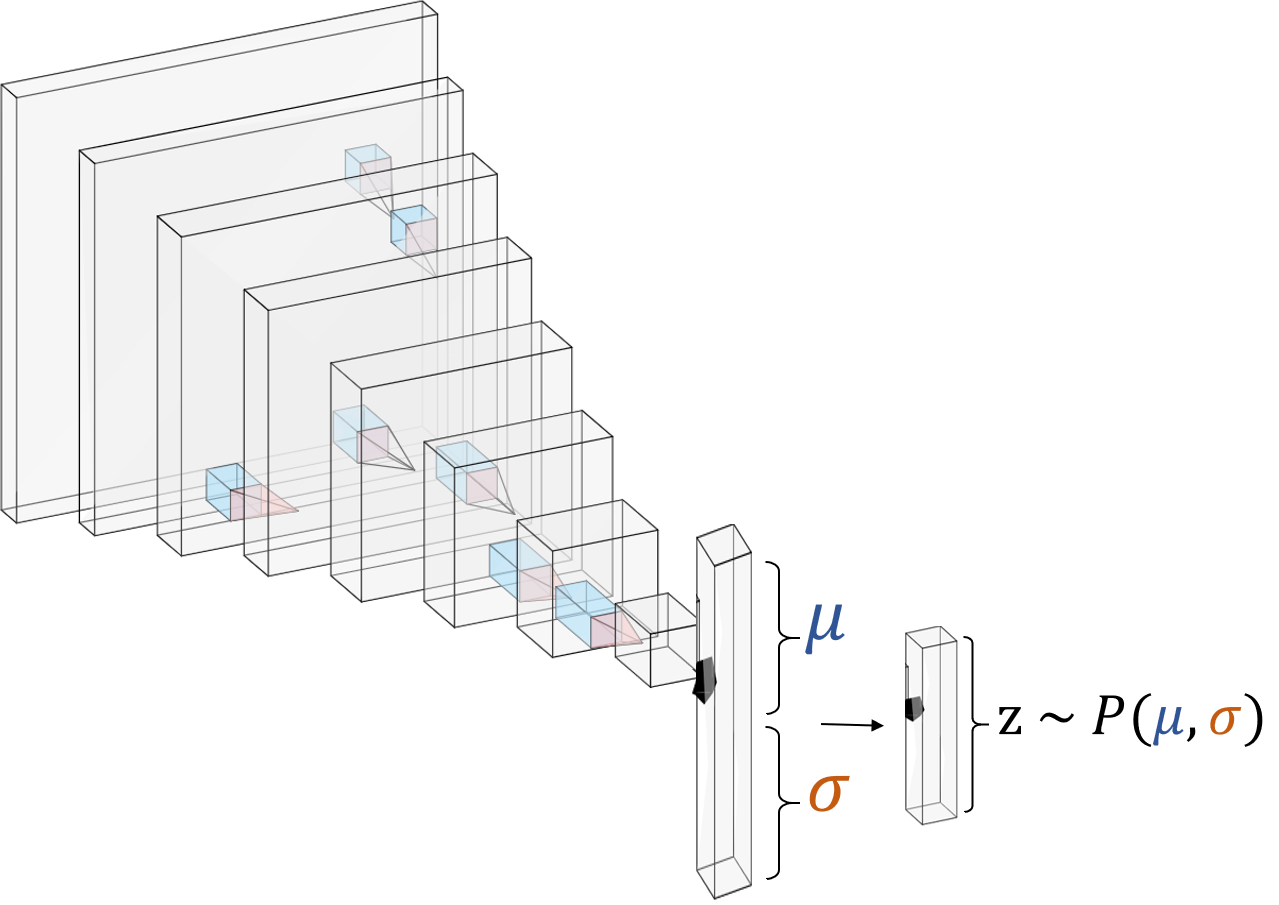
\includegraphics[scale=0.26]{figs/latent_vector.png}
                \caption{Obtención de $\mu$ y $\sigma$}
            \end{figure}
        \column{0.55\textwidth}
            \begin{itemize}
                \item Aproximación de la distribución de probabilidad de las huellas - $P(\mu,\sigma)$
                \vspace{10mm}
                \item Regularización que disminuye el overfitting del modelo.
            \end{itemize}
    \end{columns}
    
\end{frame}

% ==== SLIDE 16 ====
\begin{frame}{Trabajo futuro}

    \begin{itemize}
        \setlength\itemsep{5mm}
        \item Iterar para encontrar el equilibrio de parámetros de la divergencia KL que permita obtener un mejor desempeño del modelo.
        \item Desarrollo de algoritmos más sofisticados para el deterioro artificial teniendo como referencia modificaciones reales en las huellas.
        \item Utilizar la binarización proporcionada por el SDK de NeuroTec como la imagen objetivo de la reconstrucción.
    \end{itemize}

\end{frame}

% ==== SLIDES REFERENCIAS ====
\nocite{*}
\begin{frame}[allowframebreaks]{Referencias}
\bibliographystyle{unsrt}
\bibliography{referencias.bib}
\end{frame}

% ==== ANEXO 1 ====
\begin{frame}{ANEXOS - Entrenamiento del modelo}

     Configuración del algoritmo de entrenamiento:
     \vspace{5mm}
     
     \begin{itemize}
        \item Batch size: 48
        \item Optimizador: ADAM.
        \item Beta 1: 0.5
        \item Beta 2: 0.999
        \item Tasa de aprendizaje: 0.00018
        \item $\alpha:$ 40
        \item Épocas: 96
    \end{itemize}
    
\end{frame}

% ==== ANEXO 2 ====
\begin{frame}{ANEXOS -  Convolución y convolución Transpuesta}

    Lógica de la operación de convolución y convolución transpuesta en dos dimensiones aplicada a una imagen.

    \begin{figure}
        \begin{subfigure}{0.45\textwidth}
            \centering
            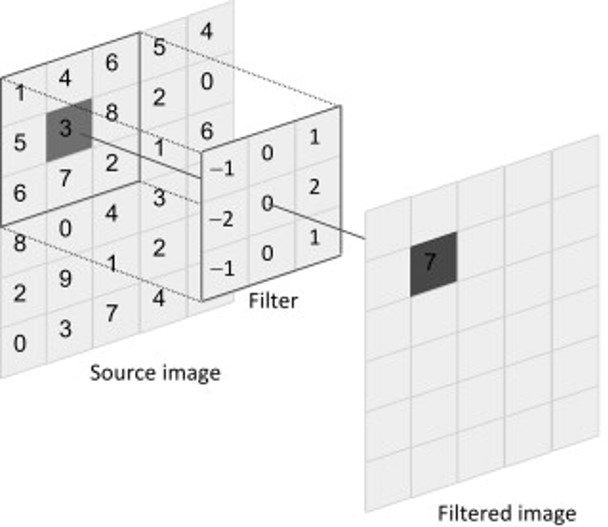
\includegraphics[scale=0.325]{figs/conv_2d.jpg}
            \caption{Convolución}
        \end{subfigure}
        \begin{subfigure}{0.45\textwidth}
            \centering
            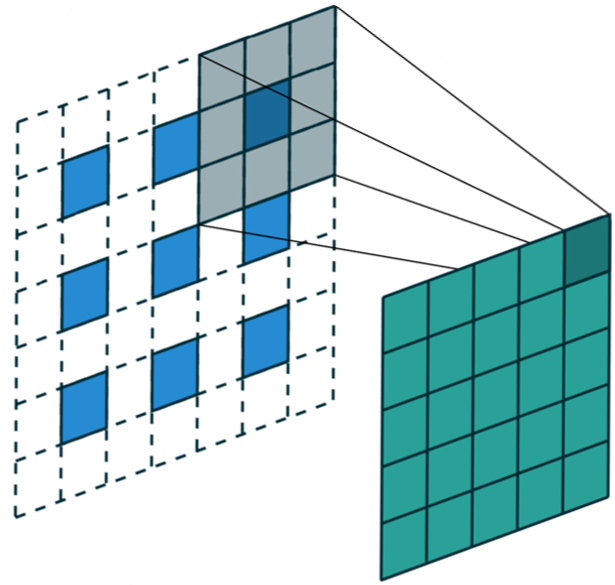
\includegraphics[scale=0.30]{figs/trans_conv.PNG}
            \caption{Convolución transpuesta}
        \end{subfigure}
    \end{figure}

\end{frame}

% ==== ANEXO 3 ====
\begin{frame}{ANEXOS - Parámetros}
    Modelo convolucional: 15 millones\\
    Perceptrón multicapa: 1000 millones
\end{frame}

\end{document}